\begin{frame}
  \frametitle{\problemtitle}
  \begin{block}{Problem}
    Find all reachable squares on an $n\times n$ grid that can be reached
    starting from the corner while alternating between knight moves of type
    $(a,b)$ and $(c,d)$.
  \end{block}
  \pause
  \begin{block}{Solution}
    \begin{itemize}
      \item Create two copies of the grid, one for ``the last move was of type
        $(a,b)$'' and one for ``the last move was of type $(c,d)$.
      \item Starting from the two top left corners, run BFS or DFS to find the reachable states.
        After each move, transfer over to the other grid.
      \item Count all cells that are reachable in at least one of the grids.
      \item Total time: $\mathcal{O}(n^2)$.
    \end{itemize}
  \end{block}
  \pause
  \solvestats
\end{frame}
\begin{frame}
  \frametitle{\problemtitle}
  
\includegraphics[width=3.4cm]{60-pretty}
  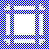
\includegraphics[width=3.4cm]{61-pretty}
  
\includegraphics[width=3.4cm]{62-pretty}
  
\includegraphics[width=3.4cm]{63-pretty}
  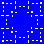
\includegraphics[width=3.4cm]{64-pretty}
  
\includegraphics[width=3.4cm]{65-pretty}
  
\includegraphics[width=3.4cm]{67-pretty}
  
\includegraphics[width=3.4cm]{68-pretty}
\end{frame}
\begin{frame}
  \frametitle{\problemtitle}
  
\includegraphics[width=3.4cm]{69-pretty}
  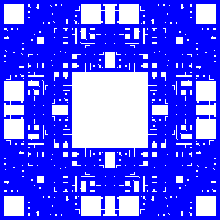
\includegraphics[width=3.4cm]{71-pretty}
  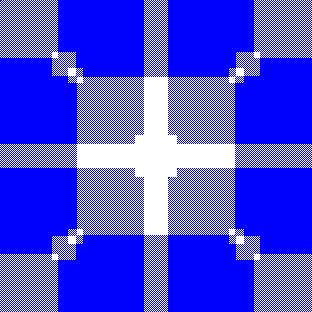
\includegraphics[width=3.4cm]{72-pretty}
  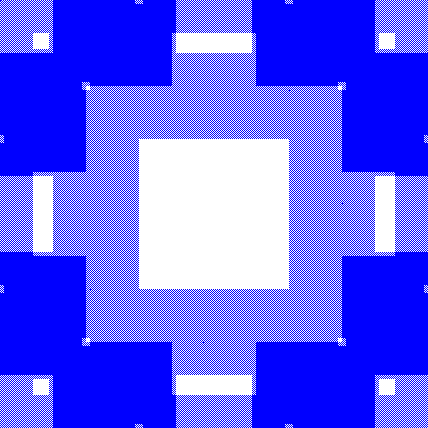
\includegraphics[width=3.4cm]{73-pretty}
  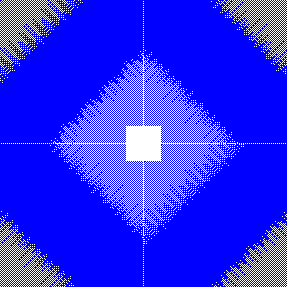
\includegraphics[width=3.4cm]{74-pretty}
  
\includegraphics[width=3.4cm]{75-pretty}
  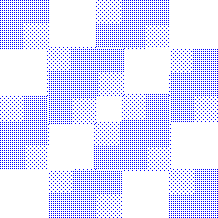
\includegraphics[width=3.4cm]{76-pretty}
  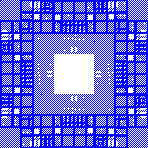
\includegraphics[width=3.4cm]{78-pretty}
\end{frame}
\begin{frame}
  \frametitle{\problemtitle}
  
\includegraphics[width=6.8cm]{70-pretty}
  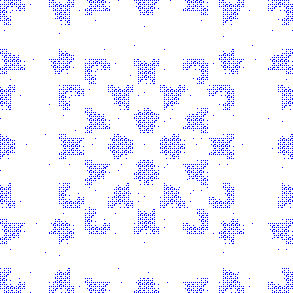
\includegraphics[width=6.8cm]{77-pretty}
\end{frame}
